\documentclass[a4paper,12pt]{article}


% % % % % % % % % % % % % % % % % % % % % % % % % % % % %
% % ATTENTION : dans les figures le label doit être mis 
%APRES le caption pour que le numéro de la figure lorqu'on
%la référence soit le bon ; sinon on a le numéro du paragraphe
% % % % % % % % % % % % % % % % % % % % % % % % % % % % %

% package qui fournit \justify 
\usepackage[document]{ragged2e}

%pifont pour les puces de formes spéciales
\usepackage{pifont}

% césure exemple
% \hyphenation{an-ti-cons-ti-tu-tion-nel

\usepackage[utf8x]{inputenc}
\usepackage[T1]{fontenc}
\usepackage[frenchb]{babel} % If you write in French
%\usepackage[english]{babel} % If you write in English
\usepackage{lmodern} % Pour changer le pack de police
\renewcommand*\familydefault{\sfdefault}
\usepackage{makeidx}
\usepackage{amsthm}
\usepackage{amsmath}
\usepackage{amssymb}
\usepackage{mathrsfs}
\usepackage{stmaryrd}
\usepackage{geometry}
%\usepackage{graphicx}
\usepackage{graphbox}
\usepackage{supertabular}
\usepackage{tabularx}
\usepackage{longtable}
\usepackage{pdflscape}
\geometry{hmargin=2cm,vmargin=2cm}

\usepackage{booktabs}
\usepackage{tabularx}
\usepackage[table]{xcolor}
\usepackage{ltablex}
\usepackage{float}
\usepackage{url}

\usepackage{chngcntr}
\counterwithin*{footnote}{page}


\usepackage[titletoc,toc,title,page]{appendix}
\renewcommand{\appendixtocname}{Annexes}
\renewcommand{\appendixpagename}{Annexes}

\usepackage{standalone}
\usepackage{ifthen}
\usepackage{xstring}
\usepackage{calc}
\usepackage{pgfopts}
\usepackage{tikz}
\usetikzlibrary{positioning,shapes,shadows,arrows}

\usepackage{algpseudocode}
\usepackage{algorithm}
\makeatletter
\renewcommand{\ALG@name}{Algorithme}
\renewcommand{\listalgorithmname}{Table des algorithmes}

\newtheorem{theo}{Définition}[section]
\usepackage{mathtools, bm}
\usepackage{amssymb, bm}

\usepackage{hyperref}
\hypersetup{
    colorlinks=true,       % false: boxed links; true: colored links
    linkcolor=black,       % color of internal links
    citecolor=purple,       % color of links to bibliography
    urlcolor=blue          % color of external links
}

\usepackage{listings}

\definecolor{dkgreen}{rgb}{0,.6,0}
\definecolor{dkblue}{rgb}{0,0,.6}
\definecolor{dkyellow}{cmyk}{0,0,.8,.3}

\lstset{
  language        = php,
  basicstyle      = \small\ttfamily,
  keywordstyle    = \color{dkblue},
  stringstyle     = \color{red},
  identifierstyle = \color{dkgreen},
  commentstyle    = \color{gray},
  emph            =[1]{php},
  emphstyle       =[1]\color{black},
  emph            =[2]{if,and,or,else},
  emphstyle       =[2]\color{dkyellow}}

%\usepackage{listings}
%\definecolor{darkgreen}{rgb}{0, 0.6, 0}
%\lstset{language = caml, frameround = fttt}
%
%\lstset{upquote=true,
%        columns=flexible,
%        keepspaces=true,
%        breaklines,
%        breakindent=0pt,
%        basicstyle=\ttfamily,
%        breaklines=true,
%        keywordstyle=\color{red},
%        commentstyle=\color{darkgreen},
%        tabsize=2,
%        escapebegin=\color{gray},
%}
\usepackage{blindtext}
\usepackage{enumitem} % pour changer les puces dans \itemize

%\author{Florian Barbarin \\ Abdelkader Beldjilali \\ Alexis Letombe\\ \\ \\ %\\Encadrant : Cyril Allignol\\ \\ \\}

% 
\includegraphics[width=0.6\textwidth]{images/enac}\\[1cm]
\date{\today}

\makeindex
\def\siecle#1{\textsc{\romannumeral #1}\textsuperscript{e}}
\newcommand{\argmax}{\mathop{\mathrm{argmax}}\nolimits}
\newcommand{\pgcd}{\mathop{\mathrm{pgcd}}\nolimits}

\makeatletter
\renewcommand{\pod}[1]{\allowbreak\mathchoice
  {\if@display \mkern 18mu\else \mkern 8mu\fi (#1)}
  {\if@display \mkern 18mu\else \mkern 8mu\fi (#1)}
  {\mkern4mu(#1)}
  {\mkern4mu(#1)}
}


\begin{document}
\renewcommand{\labelitemi}{\textbullet}
% pour factoriser l'échelle des figures 
%utilisation scale=\scaledvwa au lieu de scale = 0.3 ... 
\newcommand{\scaledvwa}{0.4} 
\newcommand{\scaledvw}{0.3}
\newcommand{\scalekad}{0.45}

%\thispagestyle{empty}
\phantomsection
\begin{titlepage}
\parindent=0pt

%www.devoloppez.com \hspace*{\stretch{1}} \LaTeX intermédiaire%

%Rubrique \LaTeX\hspace*{\stretch{1}} Tutoriels

\vspace*{\stretch{1}}
\begin{center}

\includegraphics[scale=0.5]{images/enac.png}%
\end{center}

\vspace*{\stretch{1}}
\hrulefill
\begin{center}\bfseries\Huge
    Analyse stratégique du fret aérien à l'aide du modèle des 5 forces de Porter 
\end{center}
\hrulefill

\vspace*{1cm}
\begin{center}\bfseries\Large
Nicolas Hovoet - Florian Barbarin - Abdelkader Beldjilali
\end{center}
    
%\begin{center}\bfseries\Large
%Sous la direction du Dr. Hachichi Assia et du Pr. Hajnal Ladislas
%\end{center}

    \vspace*{\stretch{2}}


\begin{flushright}
       Le \today 
\end{flushright}   

\begin{tikzpicture}[remember picture, overlay]
 \begin{scope}[shift={(current page.south west)},shift={(1,1)},scale=1]
 \shade[ball color=blue,opacity=.6] (0,0) circle (10ex);
 \shade[ball color=blue,opacity=.8] (1.7,1) circle (5ex);
 \shade[ball color=blue,opacity=.8] (1.5,3) circle (2ex);
 \shade[ball color=blue,opacity=.5] (-0.5,3) circle (1ex);
 \shade[ball color=blue,opacity=.8] (1,4) circle (1ex);
 \shade[ball color=blue,opacity=.6] (3.5,2.5) circle (2ex);
 \shade[ball color=blue,opacity=.8] (2.5,4.5) circle (4ex);
 \shade[ball color=blue,opacity=.5] (3,4) circle (3ex);
 \shade[ball color=blue,opacity=.8] (4.5,4.5) circle (3ex);
 \shade[ball color=blue,opacity=.5] (5.1,4.7) circle (2ex);
 \shade[ball color=blue,opacity=.8] (5,6) circle (1.5ex);
 \shade[ball color=blue,opacity=.6] (3.5,5.5) circle (2ex);
 \shade[ball color=blue,opacity=.8] (5,3) circle (1ex);
 \end{scope}
 \end{tikzpicture}
\end{titlepage}

%on créé la couverture

\pagebreak

\tableofcontents
\justify

\pagebreak

\section{Introduction}

Le transport aérien de fret s'est développé à partir de 1911 où un
premier vol a consisté à livrer 15 kg de courrier entre deux villes asiatiques
distantes de 10 km sur une biplan Sommer. Depuis, le traffic a légèrement augmenté pour
atteindre en 2014, 51 millions de tonnes pour une valeur de US\$6.8 trillions \cite{RePEc:eee:jaitra:v:61:y:2017:i:c:p:34-40}.
Aujourd'hui, le fret aérien joue un rôle majeur dans l'économie et le développement international.

 
La présente étude vise à effectuer une analyse de marché suivant le modèle des 5 forces de Porter,
suivie d'une étude du rôle de l'Air Traffic Management (ATM) dans la stratégie des acteurs du secteur.
Pour terminer, on s'interrogera sur l'évolution future du rôle de l'ATM au regard de ces stratégies. 
   





\subsection{Concurrence entre les firmes existantes}

\subsubsection{Définition du marché}

Le marché concerne le fret aérien qui désignera dans la suite tous les biens y compris le fret postal à l’exception des bagages.(IATA)

Cette étude porte sur les sociétés de Fret Aérien Civil Traditionnelles (FACT) qui gèrent leur propre flotte aérienne pour le transport de biens. Ce qui exclus le fret militaire ainsi que les logisticiens, entreprises de fret "virtuelles", qui font souvent du point à point par le biais de location de charters ou d'achat d'emplacements aux compagnies de fret traditionnlles. Les compagnies virtuelles constituent donc à la fois des clients pour le Fret Aérien Civil Traditionnel (FACT) qui permet à ces dernières d'optimiser le remplissage de leurs avions-cargo, mais aussi une forme de concurrence puisque le fret transporté au nom du logisticien est "perdu" pour tous les transporteurs classiques, y compris celui qui assure réellement le service. 



\subsubsection{Description des produits concernés}
Pour évaluer la concurrence, il convient d'étudier en premier lieu, le type de produits transportés. En effet, le pétrole ou le gaz, ne sont pas en général, transportés par avions ; sur ces matières premières, le fret aérien ne concurrence pas les secteurs maritimes, routiers, ferrovières, fluviaux ou par oléoduc/gazoduc. 

Le fret aérien, pour être compétitif, concerne donc les produits à haut rapport valeur-poids, souvent aussi à forte valeur ajoutée, ou à forte contrainte temporelle :


\begin{itemize}
	\item Electronique,
	\item Produits périssables : fleurs, fruits, ...
	\item Produits urgents ou à finalités humanitaires.
\end{itemize}



\subsubsection{Taxonomie des acteurs du transport du fret}

On distingue 3 types de sociétés de transport qui exhibent des structures de coûts, des ca\-racté\-risti\-ques opérationnelles et une répartition spatiale de l'offre et de la demande distinctes. En particulier, le transport en soute peut-être facturé au coût marginal car les coûts directs d'exploitation du vol sont imputés aux passagers. Le fret en soute possède donc un avantage concurrentiel sur le tout-cargo. Trois solutions possibles à ce problème, la régulation des prix pour protéger les freighters, le ré-ajustement de la flotte pour les compagnies mixtes qui revendent leur cargo, voire constituent des filiales disjointes, ou la différentiation en offrant des services spécifiques à leur clients pour les entreprises tout cargo qui ne sont pas astreintes à opérer sur des aéroports destinés au traffic passager ; il s'agit ici de tirer partie
de la souplesse dans la localisation et la topologie du réseau mondial de hubs de fret.
Les compagnies mixtes sont soumises à une barrière de sortie du secteur du fret "tout-cargo" beaucoup plus souple et rentable. Les tout-cargo, quant à elles, n'ont d'autres choix que le rachat par un concurrent ou nouvel entrant, de mettre la clé sous la porte ou de fusionner. Des alliances permettent des économies d'échelles et des synergies bénéfiques en terme de qualité et versatilité des services proposés au clients.



Les \textit {"freighters"} qui possèdent une flotte d'avions cargo dédiés qui vont du gros porteurs B747-8F de rayon d'action 8000 km et de capacité 140 tonnes, au Beluga AirBus A300 reconverti jusqu'au simple twin turboprop Cessna super cargomaster (RA : 1700 km, capacité fret : 1.8 tonnes) Ainsi, un transporteur tout\-cargo de fret classique comme Cargolux a très peu de frais de personnel et de frais commerciaux. En revanche, les coûts liés aux avions, aux redevances aéronautiques et aux frais d’escale sont élevés. En 2014, la part de marché en valeur, en revenu tonne kilomètre global (RTK), pour ce type de compagnies se monte à 56 \%. La tendance depuis 2000 est à la baisse au profit du transport en soute avec probablement, une part de marché en quantité qui ne dépasse pas désormais les 30 \%. L'adverbe \textit{probablement} souligne ici la difficulté d'obtention et d'interprétation des données aéronautiques. Les freighters sont en outre confrontées au problème de la \textit{bi-directionnalité} c'est à dire au retour à vide après livraison, spécifité qui n'existe pas dans le transport de passagers. 
	
Les \textbf{compagnies mixtes} telles que Lufthansa, Air France-KML utiliseront soit le transport en soute dans leurs avions-passagers, soit des avions cargo combinés, i.e. avions configurés de manière permanente pour le transport de fret et de PAX, soit des avions reconfigurables rapidement pour les deux types de transport. Pour illustrer le transport en soute, on note qu'un moyen-courrier assurant un vol avec 200 passagers représente un revenu d’environ US\$100 000, auxquels s’ajouteront quelque US\$13000 en fonction du taux de remplissage des soutes de l’avion. Un moyen-courrier de la catégorie A330/B767 permet d’embarquer environ 10 tonnes de fret hors bagages. En 2015, la valeur moyenne de chaque kilo transporté par avion s’établit à US\$127, contre US\$1,10 pour le maritime.
Certaines compagnies mixtes possèdent des filiales spécialisées dans le cargo. On peut citer British Airways World Cargo classée 12ème en terme de freight tonne-kilomètres (FTK). Mais même dans ce contexte, British Airways
va cessé l'exploitation de ses Boeing 747-8F. Source : \url{http://www.economist.com/node/21600946#print}
	
Les \textbf{intégrateurs}\label{integrateur} comme FedEx, UPS, TNT, qui font du point à point via des hubs dédiés, sont des entreprises avec des frais de personnel plus élevés et des coûts avion moindres grâce à une flotte d'appareils d’occasion convertis en cargo : A300-600, A310. \cite{lantenne}


\subsubsection{Description du marché}
Le fret aérien génère un chiffre d’affaires annuel évalué par l’Association internationale du transport aérien (IATA) à 47,8 milliards de dollars en 2016. Les avions ont embarqué 53,9 millions de tonnes de fret en 2016. L’aérien ne représente qu’un faible pourcentage du volume du fret (environ 5 \%),
mais environ 35 à 40 \% en valeur. \cite[lantenne]. Ce secteur demeure toutefois une activité minoritaire au sein des compagnies aériennes, le transport de passagers produisant 80 à 85 \% de ses recettes. Le transport maritime constitue le principal concurrent de l’aérien. Du fait de son coût très faible, les entreprises optimisent leur logistique pour rendre comptatible les délais de transport par mer compatibles avec leur activité. Les autres modes de fret, a contrario, se présentent parfois comme complémentaires de l'aérien : fret camionné de Toulouse au hub de Roissy-CDG par exemple.


En terme de taille de marché, on comptait en 2015 environ 200 firmes spécialisées dans le cargo, y compris les intégrateurs définis § \ref{integrateur}, auquel s'ajoute un nombre approximatif de 1100 compagnies aériennes dédiées au transport de passagers et appelées de plus en plus à alimenter l'offre en fret AFTK (Available Fret Konne-Km) ; les "Wide-Body" aux capacités en soute augmentée n'y sont pas étrangers.

Pour donner une idée, de la répartition des acteurs sur le marché, à défaut de pouvoir obtenir des données plus précises, on remarque en 2014 la prédominance des intégrateurs FedEx (7 Millions de tonnes transportés) et UPS (4 Mt) et des compagnies asiatiques et du moyen-orient, hub des pays du golf : Emirates, Korean Air, Cathay Pacific Airways à Hong-Kong. Sources : \url{http://aircargoworld.com/freight-50-the-top-50-cargo-carriers/} 

L'évolution du marché est caractérisé par une croissance molle au niveau global et un contraste géographique marqué dû notamment aux hub du Moyen-Orient et d'Asie. Sans développer davantage, on peut noter que la croissances du fret et du traffic passagers dans ces régions induit un accroissement du surplus de l'offre en fret (AFTK). Chaque mise en service d'un Boeing 777 ajoute 25 tonnes de fret 
à l'offre déjà surdimensionnée grévant ainsi la santé global du secteur. Sources : \url{http://www.economist.com/node/21600946#print}


Au niveau stratégique, le secteur est confronté à divers facteurs : sécurité, environnement, politiques protectionnistes ... On citera pour finir l'importance
de l'évolution de l'offre aéroportuaire pour éviter les problèmes de congestion.
Le climat peut en être une cause avec un nombre croissants d'aéroport inondables : 40 en Europe, 20 rien qu'en Norvège.


\subsection{Clients}


Les 10 premiers marchés de fret aérien en 2016 
(en millions de tonnes)
Etats-Unis  	7,7
Allemagne 	4,1
Chine  	3,4
Hong Kong	3,2
Japon	2,9
Emirats arabes unis 	2,4
Corée du Sud 	1,9
Royaume-Uni 	1,8
Inde  	1,6
Pays-Bas 	1,5
Source : Iata
\subsection{Fournisseurs}

Comme pour toutes les compagnies aériennes, la volatilité et le niveau des prix du pétrole est un souci permanent, compensable cependant par des investissements financiers et les solutions alternatives, réacteur à gaz ou à biocarburant, qui ne sont encore qu'à l'état de prototypes. Les contraintes réglementaires et environnementales imposent également de renouveler les flottes avec des avions plus récents.

Au niveau des constructeurs d'avions, les entreprises de fret sont, peu ou prou, confrontées au duopole Boeing - Airbus. Elles possèdent malgré tout d'une part un pouvoir de négociation proportionnel à leur taille et d'autre part la possibilité de se fournir sur le marché de l'occasion ou de faire appel à la location.

Le secteur du fret est un consommateur captif vis-à-vis des fournisseurs de services aéroportuaires. Les contraintes de volume et de poids imposent des équipements spécifiques permettant de garantir une manutention sûre et efficace, aussi bien pour les phases de (dé)chargement que par l'utilisation d'enceintes à rayons X adaptées. Les sociétés de fret sont aussi dépendantes des créneaux qui lui sont attribués et doivent faire face à la congestion du trafic en travaillant avec les différents acteurs aéroportuaires et de l'ATM. Ceux-ci peuvent alors être perçus comme des compléments auxquels il est difficile de s'abstraire totalement, bien qu'il soit possible dans un premier temps d'opérer tout ou partie d'une plate-forme aéroportuaire dédiée au fret.

Enfin, les compagnies de cargo doivent, pour rester attractives face aux compagnies mixtes et aux intégrateurs, contracter des accords avec des logisticiens pour proposer des services annexes tels que le transfert routier.
\subsection{Menaces d'éventuels entrants}

Pour les intégrateurs, les barrières à l'entrée semblent davantage relever de la présence de mastodontes tels que FedEx, UPS, TNT ou DHL capables de pratiquer des prix bas dûs aux économies d'échelles et disposant d'une forte intégration internationale et locale avec des hubs et maillages routiers optimisés. 


En outre, si la possibilité de louer ses avions plutôt que de les acheter permet de créer des compagnies ariennes fussent-elles éphémères, la sur-capacité actuelle de l'offre favorise plutôt la sortie que l'entrée. Si la demande est destinée à augmenter, la capacité l'est également avec le nombre croissant de \textit{wide-body} en circulation. Les compagnies souhaitant expérimenter le modèle mixte devront ainsi justifier d'un solide réseau de routes et de hubs, ce qui explique aujourd'hui la prépondérance des majors dans ce marché.  

A priori, les nouveaux entrants éventuels se porteront plutôt sur des marchés de niche, à moins qu'ils ne surfent sur l'apport de nouvelles technologies telles que les drones, les avions sans pilotes, le tout numérique pour réduire le coût des formalités et les accélérer, le centraliser. Mais alors les firmes en place ne sont-elles pas les mieux placées pour tirer partie de ces avancées quitte à racheter ces start-up ?
\subsection{Menaces liées à l'existence de substituts}

L'augmentation des coûts de productions à l'étranger, le développement du protectionnisme avec la crise, les problématiques liées au respect de la propriété intellectuelle constituent autant de raison pour les entreprise de relocaliser leur production. En ce sens, le transport terrestre redevient un concurrent sérieux. 


\section{Rôle de l'ATM dans la stratégie des acteurs du fret aérien}

%Single European Sky ATM Research (SESAR)

Du fait des spécificités propres au secteur du fret aérien, l'ATM joue un rôle important dans l'organisation et la stratégie des différents acteurs. En effet, nous allons voir que le fait de transporter des marchandises implique des problématiques parfois bien différentes de celles du transport de passagers.

\subsection{Un trafic réparti}

\subsubsection{Des vols ayant principalement lieu la nuit}

Comme le montre différents articles tels que \cite{popescu}, le fret aérien a, dès ses origines, été principalement organisé avec des vols ayant lieu la nuit. En effet, cela a plusieurs avantages du point de vue de l'organisation du trafic aérien. 

Tout d'abord, cette activité étant en grande partie organisée autour de grands hubs \cite{Walcott201764}, cela permet aux marchandises de transiter le jour vers ces centres névralgiques pour ensuite être redistribuées dans le monde entier dans des avions chargés en toute fin de journée. 

Ensuite, les marchandises n'étant pas soumises aux mêmes contraintes temporelles que les passagers, leur transport dans des vols de nuit permet de répartir le trafic tout au long d'une journée : les heures de pointe sont alors consacrées aux vols passagers et les créneaux disponibles la nuit aux vols cargo. Cela permet donc de ne pas rajouter de trafic lors de périodes de congestion puisque les marchandises peuvent, dans la plupart des cas, partir en plein milieu de la nuit.

Une organisation de nuit peut également permettre à des entreprises de transport de fret de réduire certains coûts et d'assouplir leur organisation. En effet, ces vols ayant lieu hors période de congestion, les redevances aéroportuaires et de contrôle aérien peuvent être moins élevées qu'en plein pic de trafic. De même, la demande étant moindre, l'allocation de créneaux s'en trouve grandement facilitée.

Enfin, cette organisation autour de vols de nuit permet à certains acteurs de diversifier leur activité. On peut citer en France l'exemple de ASL Airlines France (anciennement Europe Airpost) qui possède plusieurs B737-300 \textit{Quick-Change} lui permettant d'effectuer des vols passagers le jour et des vols de fret la nuit.\\

On voit donc que les différents acteurs du transport aérien de fret prennent en considération un certain nombre de problématiques liées à l'organisation générale du trafic aérien et décident alors d'organiser principalement leur activité la nuit. Nous allons cependant voir que d'autres problématiques ATM peuvent porter atteinte à ce mode de fonctionnement.

\subsubsection{Un trafic de nuit remis en cause}

Comme nous venons de le voir, les transporteurs aériens de fret utilisent essentiellement des créneaux de nuit pour leurs vols. Cependant, principalement pour des raisons de gêne des riverains, le trafic de nuit est remis en cause sur de nombreux aéroports. Par exemple, un couvre-feu est mis en place sur l'aéroport de Paris-Orly entre 23H30 et 6H00 depuis 1963 afin d'éviter le survol par les aéronefs des zones habitées en plein milieu de la nuit.

Il est à noter que sur certains aéroports, le trafic de nuit peut être malgré tout important du fait de la présence du hub de certaines compagnies de fret. C'est le cas notamment à Paris-Charles-de-Gaulle où FedEx et d'autres compagnies de fret ont leur hub. 

Les articles \cite{boutelet_2012} et \cite{garric_2012} montrent par exemple en quoi la fin des vols de nuit imposée à l'aéroport de Francfort peut porter atteinte au développement du trafic de fret aérien.

Dans ce cadre, les compagnies sont dans l'obligation de revoir leur stratégie vis-à-vis de l'organisation du trafic. Les départs des vols de fret doivent alors se faire plus tôt ou plus tard et, parfois, prendre part à la congestion à certaines périodes.

Cette réduction des possibilités de vols de nuit peut également pousser les compagnies vers une réduction de l'utilisation d'avions tout-cargo au profit de l'embarquement de fret sur les vols passagers. C'est en effet une tendence forte du secteur comme le montre \cite{RePEc:eee:jaitra:v:61:y:2017:i:c:p:34-40}. Même si cette tendance ne trouve pas forcément son origine dans la réduction des vols de nuit, cette nouvelle contrainte ne fait que favoriser ce changement de stratégie. Cela permet en effet d'optimiser l'utilisation des capacités de transport des aéronefs passagers en embarquant du fret qui aurait pu être transporté par un avion tout-cargo et donc de réduire le trafic des aéronefs entièrement dédiés au fret. L'article montre même que certaines compagnies, comme Air France, éliminent les avions tout-cargo de leur flotte au profit de ce mode de transport des marchandises.

Dans le cas où les aéroports continuent de permettre les vols de nuit, les problèmes de voisinage liés à ces vols ont d'autres impacts sur la gestion du trafic. Par exemple, de nombreux aéroports ont mis en place des procédures particulières pour que la gêne des riverains soit diminuée la nuit. Il s'agit dans la plupart des cas de nouvelles procédures aux instruments plus précises, évitant le survol de certaines zone voire obligeant les aéronefs à survoler un endroit précis au-dessus d'une certaine altitude. Ces procédures mises en place montrent bien le rôle que peut avoir l'ATM pour permettre aux compagnies de fret de continuer à voler la nuit sur certains aéroports.\\

On voit donc que des contraintes liées à la gestion du trafic de nuit peuvent imposer aux compagnies de fret de se réorganiser et de redéfinir en quelque sorte leur stratégie.

\subsection{Un réseau fortement maillé}

Comme le montre \cite{O'Kelly20141}, des compagnies de transport de fret comme FedEx bénéficient de plusieurs hubs dans le monde entier et d'un réseau de lignes très dense. Cela permet donc une optimisation très fine  du trafic et des coûts au sein de chaque compagnie. Voyons les implications que cela peut avoir du point de vue de l'ATM.

\subsubsection{Un "routage" facilité des marchandises}

La densité du réseau auquel ont accès les compagnies de fret permet du multiplier les chemins permettant, à partir d'un point A, d'arriver à un point B. En effet, une marchandise de FedEx partant de France et dont la destination finale est le centre des États-Unis pourra emprunter sans grande différence en terme de distance le hub de Memphis, d'Oakland ou d'Indianapolis.

Cela permet aux compagnies d'optimiser les différents chargements de leurs avions et, par là, de répartir sur différentes lignes les marchandises transportées, mais aussi de limiter le phénomène de retour à vide. Encore une fois, cela peut avoir des implications non négligeables en terme de gestion du trafic puisqu'au lieu de faire partir plusieurs avions vers une même destination, certaines charges transportées peuvent être réparties sur d'autres lignes déjà existantes.

Cette optimisation du "routage" des marchandises est, de plus, renforcée par le point qui suit.

\subsubsection{Un trafic très résilient face aux retards}

Comme nous avons déjà pu le remarquer, le transport de marchandises a pour spécificité de ne pas avoir les mêmes contraintes temporelles que les passagers.

En effet, lorsqu'un avion transportant des passagers est en retard ou annulé, un grand nombre de mesures doivent être mises en place pour la prise en charge de ces derniers et leur acheminement dans les meilleurs délais.

En ce qui concerne la plupart des marchandises, un retard de quelques heures n'a que très peu d'implications (sauf marchandises bien spécifiques comme dans le cas du transport d'animaux vivants). Ainsi, il est possible de faire le choix de routes rallongeant quelque peu le transport d'une marchandise sans que cela ait un réel impact sur le service rendu. Cela permet encore une fois d'optimiser la répartition des marchandises sur différentes lignes.

De même, les compagnies de fret étant, dans certains cas, très résilientes face aux retards, il leur est possible d'accepter, par exemple, des changements de créneau afin de désengorger le trafic sur un aéroport congestionné.\\

On voit donc en quoi la spécificité du transport aérien de fret a des implications sur la gestion générale du trafic aérien. Nous pouvons d'ailleurs également voir qu'un certain nombre de nouveaux développements dans l'ATM peuvent encore modifier les stratégies des acteurs du fret aérien.

\newpage
\section{Injection SQL }


\subsection{Description}




L'injection SQL, en anglais SQL  injection, ou SQLi en abrégé, est une des attaques les plus dangereuses. Comme pour le Cross Site Scripting présenté dans la suite de ce document, il s'agit ici de tirer parti de l'absence de filtrage des entrées utilisateurs. Cette absence de contrôles permet à un hacker d'insérer du code qui sera interprété par l'analyseur cible, par exemple SQL.




\paragraph{}
Dans la cas particulier de l'injection SQL et du site DVWA, les requêtes SQL, imbriquées dans des scripts PHP qui récupèrent les saisies des utilisateurs, peuvent être détournées sur la base de la syntaxe du langage. 

\begin{figure}[!h]
	\begin{center}
		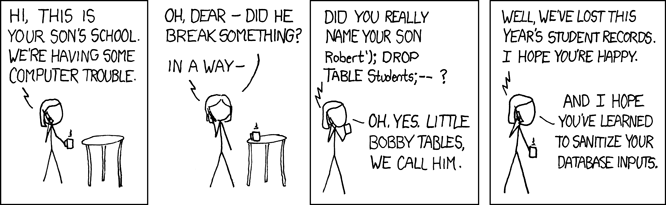
\includegraphics[scale=1]{images/bd.png}
		\caption{source : \url{https://xkcd.com/327/}}
	\end{center}
\end{figure}


\subsection{Exploitation}

\subsubsection{DVWA - Security level "low"}

La base de données contient 5 utilisateurs identifiés par les entiers de 1 à 5.
La mission proposée par le DVWA est de voler leurs mots de passe par injection SQL.

On règle la "DVWA security" sur low de manière à avoir un site web "damn vulnerable".
On saisit dans le champ User Id, une simple apostrophe i.e. '. Le site retourne le message
"\it {You have an error in your SQL syntax; check the manual that corresponds to your MariaDB server version for the right syntax to use near ''''' at line 1}"

\paragraph{}Cette simple apostrophe démontre que le site est vulnérable pour deux raisons : d'abord on sait que nos saisies sont interprétées directement par l'analyseur SQL ; elle ne sont pas filtrées. Ensuite parce que le site est "bavard".

\begin{figure}[!h]
	\begin{center}
		\label{}
		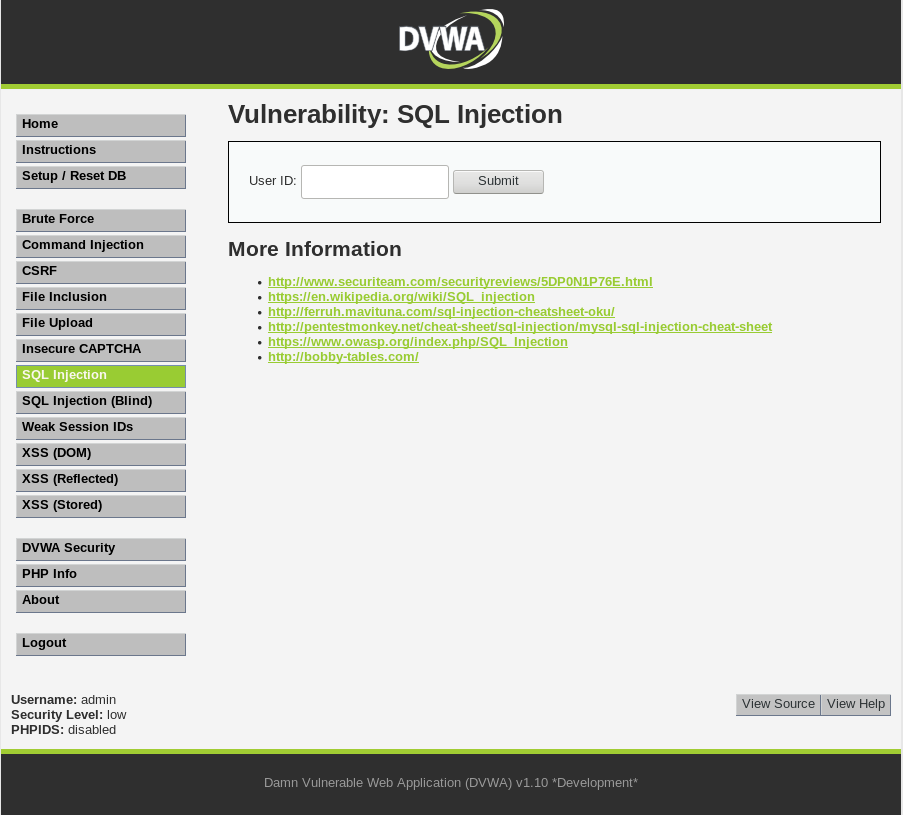
\includegraphics[scale=\scaledvwa]{images/sql/sqli1.png}
		\caption{Les saisies incorrectes donnent lieu à un message d'erreur SQL qui informe le hacker potentiel de l'absence de protection contre les SQLi. D'autres informations importantes sont dévoilées comme le type de base de donnée, ici MariaDB, version libre de MySql rachetée par Oracle.}
	\end{center}
\end{figure}

Un clic sur le bouton "View Source" affiche le code PHP de la page. On constate, en effet, qu'on peut saisir n'importe quoi dans le champ User Id, il sera transmis sans modification à la requête \$query via \$id.   

\begin{figure}[!h]
	\begin{center}
		\label{}
		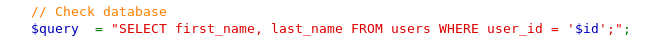
\includegraphics[scale=0.8]{images/sql/code_low.png}
	\end{center}
\end{figure}



\begin{figure}[!h]
	\begin{center}
		\label{}
		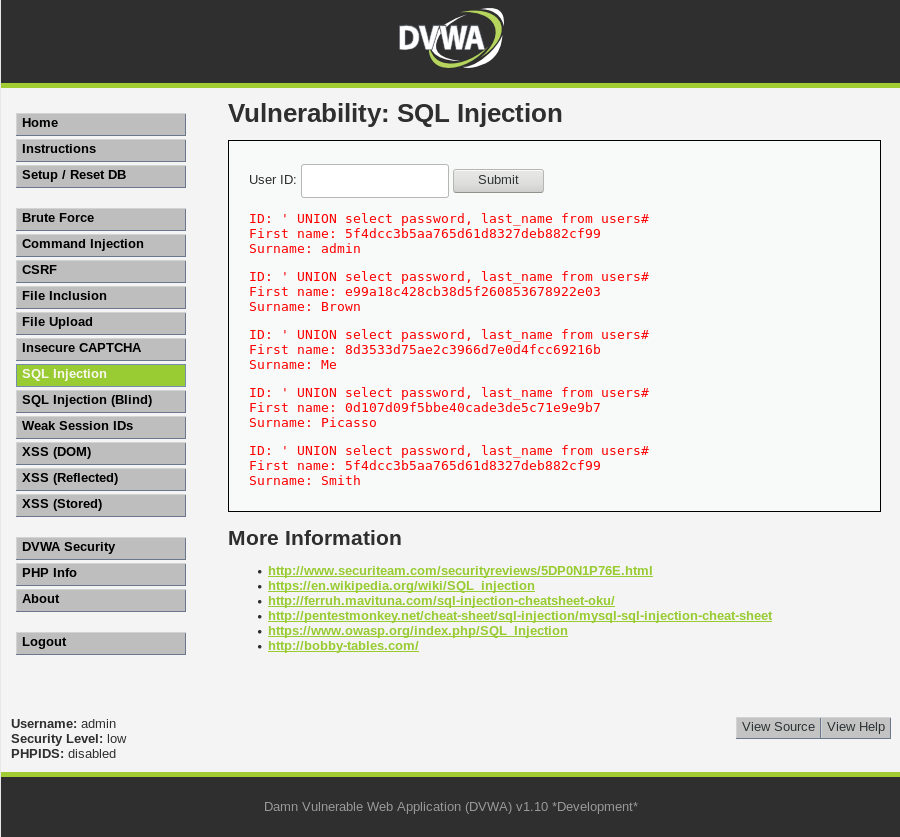
\includegraphics[scale=\scaledvwa]{images/sql/sqli_low.png}
		\caption{Vol des mots de passe par l'injection SQLi sur site non protégé.}
	\end{center}
\end{figure}

L'injection SQL suivante :
{\color{red}

\begin{verbatim}
   ' UNION select password, last_name from users#
\end{verbatim}
}

%  a' UNION SELECT password,last_name from users;-- -&Submit=Submit
% url correspondante 
%  ?id='+UNION+SELECT+password%2Clast_name+from+users%23&Submit=Submit#

donne la requête suivante en remplaçant \$id dans le script PHP :

{\color{red}
\begin{verbatim}
$query  = "SELECT first_name, last_name FROM users WHERE user_id = '' UNION 
           SELECT password, last_name from users#   ';"; 
\end{verbatim}
}
Elle indique donc qu'on effectue l'union au sens mathématique des éléments recueillis par les deux requêtes. Le premier SELECT donne l'ensemble vide, le second donne tous les mots de passe et noms de la table users. On obtient donc les mots de passe faussement associés au champ "First name". Ces mots de passe sont cryptés. On pourra utiliser des techniques de révélation par ingénieurie sociales, recherche internet, force brute, dictionnaires ou rainbow tables. L'outil John the ripper peut entrer en action. On note que Smith est certainement aussi admin car ces deux noms d'utilisateurs ont le même hash donc le même mot de passe. Le hacker peut être confiant quant à la suite des opération car Smith ne semble pas être un adepte de la SSI. Le caractère \# en fin d'injection évite que PHP n'interprête la suite du code en particulier les caractères apostrophes et guillements qui donneraient une erreur SQL.

NB : C'est une technique répandue que de forcer l'analyseur SQL à ignorer le reste de la requête, en utilisant le symbole commentaire SQL double tiret - - les symboles de commentaires PHP dièse \#, {/* */}, {//} pour assurer que ce qui suit l'injection ne sera pas interprété.  



\paragraph{}
Un injection SQL peut aussi donner accès au système de fichier comme le montre l'injection ci-après :
\begin{verbatim} [ ' UNION ALL SELECT load_file('/etc/passwd'),null # ] \end{verbatim}

\begin{figure}[!h]
	\begin{center}
		\label{}
		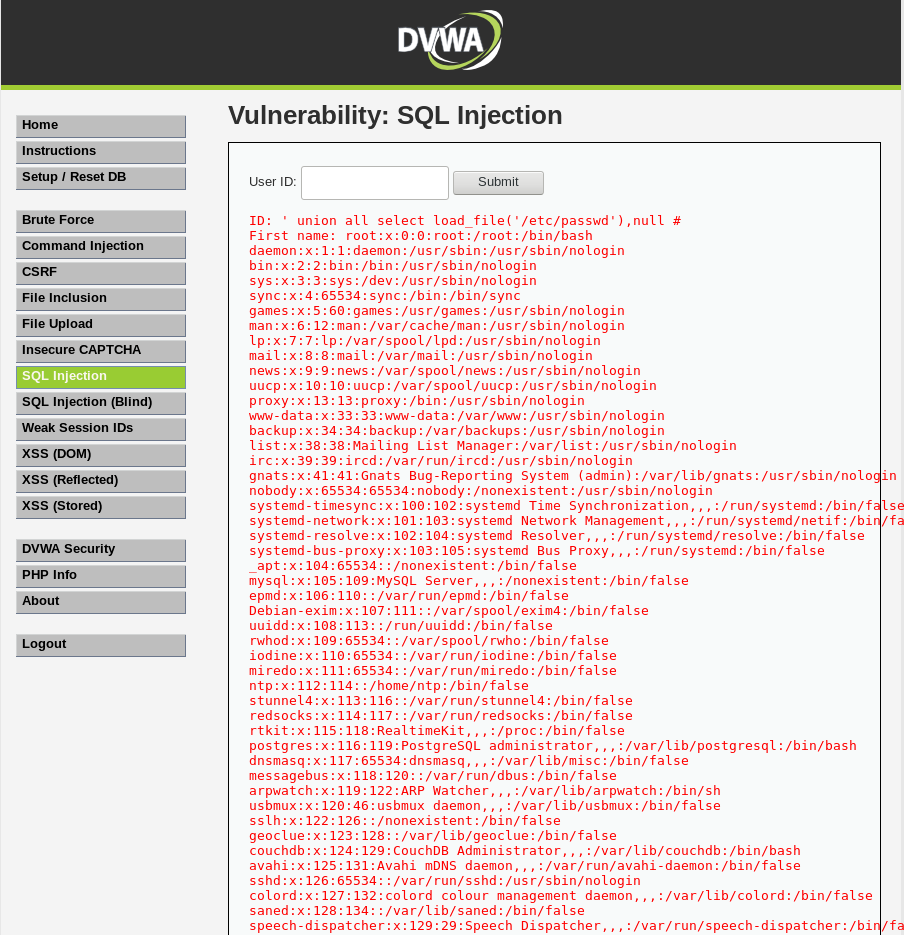
\includegraphics[scale=\scaledvwa]{images/sql/sqli_low2.png}
		\caption{Récupération du fichier /etc/passwd via la commande load\_file : }
	\end{center}
\end{figure}




% ?id=a UNION SELECT password,last_name from users;-- -&Submit=Submit
% ?id=a %27UNION SELECT password,last_name from users#


Si l’on part à la recherche des méthodes et fonctions que l’on peut utiliser en PHP afin de se protéger de certains caractères, on peut croiser le chemin de la fonction PHP mysql\_real\_escape\_string. Celle-ci est souvent utilisée pour protéger les requêtes SQL intégrant des paramètres envoyés par l’utilisateur. Néanmoins nous allons voir que cette fonction peut être déjouée, c’est d’ailleurs le but dans ce niveau DVWA.

Si l’on schématise, il faut donc faire passer des caractères comme des guillemets ou des apostrophes, sans inscrire dans l’URL les caractères en question. Un joyeux défi ! Pour ceux qui ont l’habitude de travailler sur les technos web, vous avez peut être déjà entendu parlé de l’encodage, et plus spécifiquement de l’encodage HTTP ou “HTML URL Encoding”. Pour ceux qui ne voient pas de quoi il s’agit, je vous conseille de faire un tour sur cette page : http://www.w3schools.com/tags/ref\_urlencode.asp

L’HTML URL Encoding permet entre autre de faire passer au travers une URL des caractères spéciaux ou des lettres avec accent qui pourraient ne pas être interprétés correctement par les navigateurs ou les serveurs web. Ainsi, l’utilisation d’un encodage basé sur les caractères ASCII est utilisé (notamment la valeur “Hex” des lettres : http://table-ascii.com/ )

\begin{verbatim}
En utilisant l’HTTP URL Encoding, un espace devient un %20 dans l’URL, un  “!” devient un %21, un “%” un %25, etc.

Cela nous permet donc ici de faire passer une guillemet ou une apostrophe de façon encodée pour ne pas qu’ils soient détectés et échappés par la fonction mysql_real_escape_string.
\end{verbatim}


\subsubsection{DVWA - Security level "Medium" et "High"}

Pour récupérer les mots de passe lorsque l'on règle le niveau de sécurité de DVWA sur "haut" et "medium", on utilise une combinaison des outils "Burp suite" et "sqlmap" fournis par kali linux. Le navigateur doit être configuré en utilisant ce proxy Burp suite, à savoir 127.0.0.1:8080. Cela permet l'interception des requêtes POST qui est alors copiée dans un fichier toto.txt utilisé ensuite dans la commande.

\begin{verbatim}
sqlmap -r ./toto.txt –dbs -D dvwa –dump all –os-shell
\end{verbatim}


\subsection{Contre-mesures}

Un certain nombre de règles permettent de se prémunir des attaques par injection de commandes SQL :
Pour se prémunir des injections SQL, on peut appliquer les principes suivants :
 \begin{itemize}[font=\color{magenta} \Large, label=\ding{43}]
	\item Vérifier le format des données saisies et notamment
	la présence de caractères spéciaux, 
	\item Éviter les comptes sans mot de passe,
	\item Ne pas afficher de messages d’erreur explicites affichant la requête ou une partie de la requête SQL,
	\item Restreindre au minimum les privilèges des comptes utilisés,
	\item Supprimer les comptes utilisateurs non utilisés, notamment les comptes par défaut,
	\item Utiliser un firewall Applicatif de type mod\_security
    \item Désactiver l’option Load\_File.
\end{itemize}


Plus spécifiquement, il est possible d'utiliser des "requêtes préparées" comme dans l'exemple en PHP tiré de DVWA - level "impossible"; le code et les données sont alors entièrement séparées. Une référence web utile se trouve sur le site \href{https://openclassrooms.com/courses/administrez-vos-bases-de-donnees-avec-mysql/requetes-preparees}{requetes-preparees}.
\begin{figure}[!h]
	\begin{center}
		\label{}
		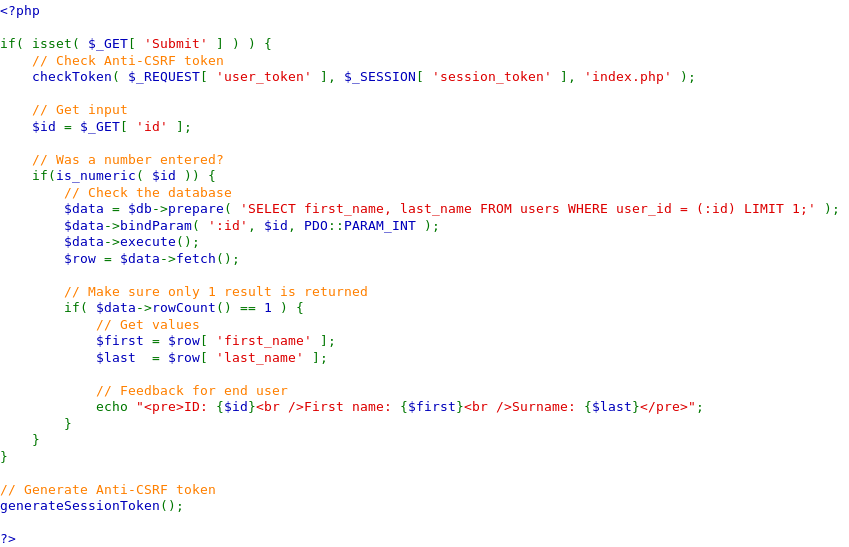
\includegraphics[scale=1]{images/sql/sqli_impossible.png}
	\end{center}
\end{figure}

























\section{Injection SQL aveugle}

\subsection{Description}

Les injections SQL aveugles, ou "blind SQL" en anglais, qu'on peut nommer BSQLi,  sont des techniques utilisées lorsque le serveur n'est pas "bavard". Sur le plan du code PHP, il suffit de retirer la ligne de code suivante qui renvoie les erreurs SQL : 
\begin{verbatim}
or die('<pre>' . mysql_error() . '</pre>' );
\end{verbatim} 



\subsection{Exploitation}

\subsection{Contre-mesure}


\section{Attaques XSS }Reflected XSS

\subsection{Description}
 désignées au choix par les acronymes CSS ou XSS et qui seront
Un site web qui fournit d'une part un service de recueille d'informations via des formulaires et d'autre part un service de publication sur le site de ces mêmes informations
\subsection{Exploitation}

\subsection{Contre-mesure}


\section{Attaques XSS enregistrées }

\subsection{Description}

\subsection{Exploitation}

\subsection{Contre-mesure}


















%
%
%@ARTICLE{1056964,
%	author={A. Shamir},
%	journal={IEEE Transactions on Information Theory},
%	title={A polynomial-time algorithm for breaking the basic Merkle-Hellman cryptosystem},
%	year={1984},
%	volume={30},
%	number={5},
%	pages={699-704},
%	keywords={Cryptography;Computer science;Graphics;Mathematics;Microcomputers;Polynomials;Protection;Public key;Public key cryptography;Security;Testing},
%	doi={10.1109/TIT.1984.1056964},
%	ISSN={0018-9448},
%	month={Sep},}
%
%
%@BOOK{MARTIN2004,
%	title = {Codage, cryptologie et applications},
%	publisher = {Presses polytechniques et universitaires romandes},
%	year = {2014},
%	author = {Martin, Bruno}
%}
%
%@Book{GJ1979,
%	author = "Michael R. Garey and David S. Johnson",
%	title = "{Computers and Intractability, A Guide to the Theory of {NP}-Completeness}",
%	publisher = "W.H. Freeman and Company",
%	year = 1979,
%	address = "New York"
%}
%
%@book{opac,
%	title = "Handbook of Applied Cryptography",
%	author = "Alfred J. Menezes and Paul C. Van Oorschot and Scott A. Vanstone",
%	publisher = "CRC Press",
%	address = "Boca Raton, London, New York",
%	url = "http://opac.inria.fr/record=b1092394",
%	isbn = "0-8493-8523-7",
%	year = 1996,
%	note = {\url{http://cacr.uwaterloo.ca/hac/}}
%}
%
%@ARTICLE{DEROFF,
%	author={J. Deroff and R. Goyat},
%	title={Le problème du sac à dos en cryptographie},
%	year={2007},
%	note = {\url{http://j.deroff.free.fr/rapportter.pdf}}
%}
%
%@Book{stinson1996,
%	author =       {Stinson, Douglas},
%	title =        {{Cryptographie -- Théorie et pratique}},
%	publisher =    {International Thomson Publishing},
%	year =         {1996},
%	note =         {Traduction de Serge Vaudenay},
%}
%
%@ARTICLE{COSTER,
%	author={Coster, Matthijs J. and Joux, Antoine  and La Macchia, Brian A. and Odlyzko, Andrew M. and Schnorr, Claus-Peter and Stern, Jacques},
%	title={Improved low-density subset sum algorithms},
%	journal={computational complexity},
%	year={1992},
%	volume={2},
%	number={2},
%	pages={111-128},
%	mounth={June},
%	note = {\url{http://www.di.ens.fr/~fouque/ens-rennes/sac-LLL.pdf}}
%}
%
%@article{Merkle,
%	author = {Merkle, R. and Hellman, M.},
%	title = {Hiding Information and Signatures in Trapdoor Knapsacks},
%	journal = {IEEE Trans. Inf. Theor.},
%	issue_date = {1978},
%	volume = {24},
%	number = {5},
%	month = {Sep},
%	year = {1978},
%	issn = {0018-9448},
%	pages = {525--530},
%	numpages = {6},
%	url = {http://dx.doi.org/10.1109/TIT.1978.1055927},
%	doi = {10.1109/TIT.1978.1055927},
%	acmid = {2269393},
%	publisher = {IEEE Press},
%	address = {Piscataway, NJ, USA},
%} 

\section{Conclusion et perspectives}

\paragraph{} Bien que le problème de somme de sous-ensembles (SSP) soit NP-complet, des algorithmes peuvent être mis en place pour tenter de casser le cryptosystème de Merkle-Hellman dans sa version basique. Si les algorithmes de force brute montrent très vite leurs limites, l'apport de théories plus ou moins récentes telles que la géométrie des nombres et la notion de réseau permet d'envisager des algorithmes nouveaux et élégants, bien que leur succès soit loin d'être garanti. Enfin, tous les sacs à dos ne se valent pas. Comme nous avons eu l'occasion de le voir, certaines méthodes comme la programmation dynamique ont horreur des sacs à dos dilatés alors que la densité est l'ennemie de l'algorithme LLL. La diversité des méthodes de cryptanalyse et la difficulté de se protéger contre l'une sans s'exposer à une autre justifie pleinement l'abandon de ce cryptosystème au profit de systèmes réputés plus sûrs, du moins à l'heure actuelle, comme RSA. 

\paragraph{} Il n'en reste pas moins
que le SSP reste un problème intéressant à étudier sur le plan théorique et pratique. L'application de méthode hybrides associant les techniques de programmation dynamique et arborescentes
avec heuristiques ont fait l'objet de nombreuses publications. Enfin, appliquer des algorithmes endémiques au domaine de l'intelligence et de l'apprentissage artificielle, tels les « colonies de fourmis », les algorithmes génétiques ou les réseaux de neurones  
pourraient fournir des pistes plus innovantes.


%\newpage
%\appendix
%\section{Annexe}
\label{annexe_A}

\begin{itemize}
\item Pour écrire simplement les clés sur le disque, nous utilisons Marshal, qui garantit la compatibilité entre toutes les plateformes pour une même version de OCaml.
\item Bien que BatIO propose une API pour manipuler les canaux au niveau du bit, nous avons préféré rester au niveau de l'octet car il s'agit d'une solution plus évolutive – rares sont les bibliothèques proposant ce genre de fonctions. D'ailleurs, son fonctionnement est identique à ce que nous implémentons, reposant sur une lecture octet par octet.
\item Dans la version actuelle du code, les canaux d'entrées-sorties ne sont pas toujours fermés proprement lorsqu'une exception « fatale » est rencontrée…
\item Les blocs chiffrés sont écrits sur le canal de sortie sous forme de chaîne de caractères. Ainsi, le message chiffré constitué de deux blocs « 1234 5678 » est écrit, sous forme hexadécimale, «~31 32 33 34 00 35 36 37 38 00~». Pour déchiffrer, on lit donc le canal d'entrée « chaîne par chaîne ». Cela a l'avantage de produire une sortie lisible mais présente l'inconvénient de consommer bien plus d'espace qu'une représentation binaire qui serait spécialement conçue pour le problème.
\end{itemize}

%\section{Annexe}
\label{annexe_A}

\begin{itemize}
\item Pour écrire simplement les clés sur le disque, nous utilisons Marshal, qui garantit la compatibilité entre toutes les plateformes pour une même version de OCaml.
\item Bien que BatIO propose une API pour manipuler les canaux au niveau du bit, nous avons préféré rester au niveau de l'octet car il s'agit d'une solution plus évolutive – rares sont les bibliothèques proposant ce genre de fonctions. D'ailleurs, son fonctionnement est identique à ce que nous implémentons, reposant sur une lecture octet par octet.
\item Dans la version actuelle du code, les canaux d'entrées-sorties ne sont pas toujours fermés proprement lorsqu'une exception « fatale » est rencontrée…
\item Les blocs chiffrés sont écrits sur le canal de sortie sous forme de chaîne de caractères. Ainsi, le message chiffré constitué de deux blocs « 1234 5678 » est écrit, sous forme hexadécimale, «~31 32 33 34 00 35 36 37 38 00~». Pour déchiffrer, on lit donc le canal d'entrée « chaîne par chaîne ». Cela a l'avantage de produire une sortie lisible mais présente l'inconvénient de consommer bien plus d'espace qu'une représentation binaire qui serait spécialement conçue pour le problème.
\end{itemize}


\newpage
\nocite{*}  %affiche toutes les entrées du bib même celles qui ne sont pas citées.
% cf.    http://www.tuteurs.ens.fr/logiciels/latex/bibtex.html
% compilation en TROIS PHASE  bibtex traite un fichier *.aux mais bibtex mon_fichier comme bibtex mon_fichier.aux sont acceptés 
% latex mon_fichier.tex
% bibtex mon_fichier
% latex mon_fichier.tex


% \renewcommand{\bibname}{Toto}
% ou
\renewcommand{\refname}{Bibliographie}
% dans le préambule.
\bibliographystyle{alpha}
\bibliography{references}


\pagebreak
%\clearpage

\thispagestyle{empty}
\ThisTileWallPaper{1.45\paperwidth}{1.0\paperheight}{images/fret}


\addtolength{\wpXoffset}{-4.5cm}

\justify

%{\LARGE
%
%\color{white}{Ce rapport propose une analyse stratégique du fret aérien suiviant le modèle de Porter.}
%}

%\begin{figure}[!h]
%	\begin{center}
%		\label{}
%		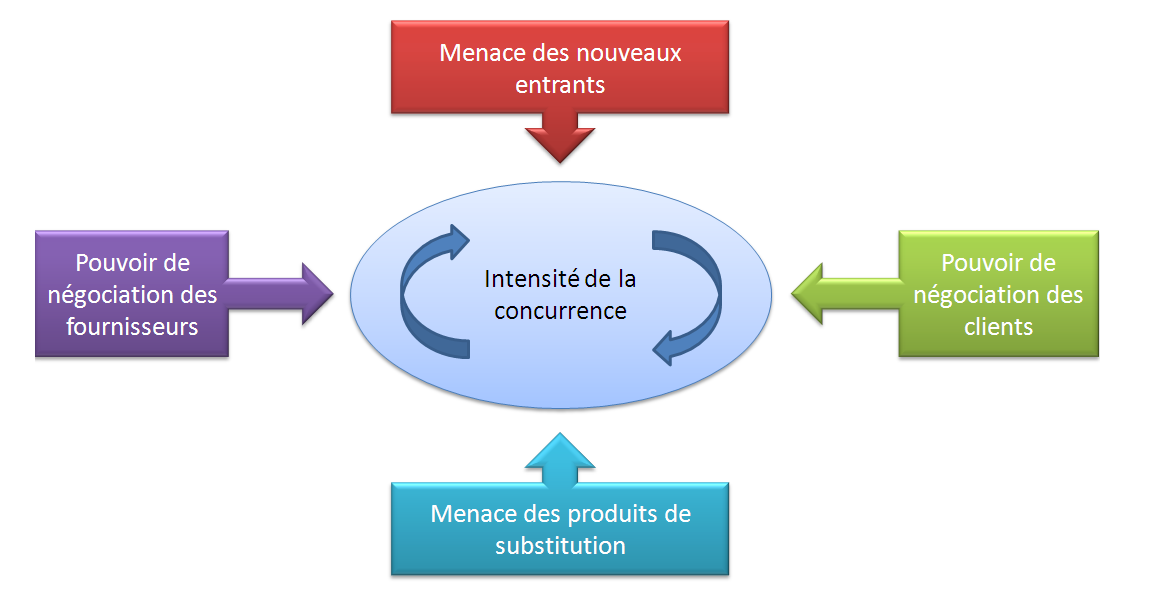
\includegraphics[scale=0.4]{images/porter/porter_2}
%	\end{center}
%\end{figure}







\end{document}
